%!TEX ROOT=formularioFisica.tex

\section{Dinamica}\label{sec:dinamica}
La dinamica è la branca della fisica che studia il moto dei corpi servendosi delle forze che ne
sono responsabili. Isaac Newton ha enunciato i principi della dinamica e in suo onore la forza é 
misurata in Newton (N).\\
Per gli esercizi si vada a pagina~\pageref{ex:dinamica}.
\subsection{Secondo Principio della Dinamica}
Una forza è una grandezza vettoriale che porta una modificazione alla velocità del corpo.
\begin{equation*}
  \vec{F} = m\vec{a}
\end{equation*}
$F$: forza applicata\\
$m$: massa del corpo\\
$a$: accelerazione\\ [\baselineskip]
Se due corpi interagiscono tra loro, si sviluppano due forze, dette comunemente azione e reazione: 
sono uguali in modulo e direzione, ma opposte in verso.\\
Un corpo è in equilibrio quando la somma delle forze è 0, $\sum F_y = 0\land\sum F_x = 0$.\\
Le forze si dividono in \emph{conservative} e \emph{dissipative}. Quando agisce una forza conservativa
l'energia si mantiene, quando una dissipativa si perde energia.\\ [\baselineskip]
Perché un corpo su un tavolo piano sta in equilibrio?
\begin{center}
  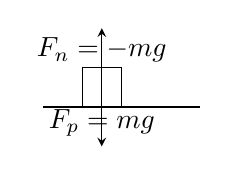
\begin{tikzpicture}
    \draw (0,0) -- (2,0);
    \draw (0.5,0) -- ++(0,0.5) -- ++(0.5,0) -- ++(0,-0.5) -- cycle;
    \draw[-stealth] (0.75,0.25) -- +(0,0.75)
      node[pos=1,below]{$F_n = -mg$};
    \draw[-stealth] (0.75,0.25) -- +(0,-0.75)
      node[pos=1,above]{$F_p = mg$};
  \end{tikzpicture}
\end{center}
Perché è presente la forza normale che ha verso opposto alla forza premente ma direzione e modulo 
uguale.

\subsection{Attrito}
Ci sono vari tipi di attrito: \emph{statico}, \emph{dinamico} e \emph{volvente} ma tutti si basano
sullo stessa idea: moltiplicare il coefficiente di attrito tra le superfici per la forza premente.
Il coefficiente di attrito rappresenta il termine di proporzionalità tra la forza di attrito e la 
forza normale con la quale una superficie agisce su un’altra superficie. Il coefficiente di 
attrito è una proprietà che caratterizza entrambe le superfici, non è una caratteristica di una 
singola superficie o di un singolo materiale.
\begin{equation*}
  F_s \leq \mu_sF_p\quad (\text{corpo fermo})
\end{equation*}
\begin{equation*}
  F_d = \mu_dF_p\quad (\text{corpo in movimento})
\end{equation*}
\begin{equation*}
  F_v = \mu_vF_p\quad (\text{corpo rotante})
\end{equation*}
$F_p$: forza premente

\subsection{Piano Inclinato}
In un piano inclinato la forza peso fa andare in basso il copo se $P_\| > \mu_s\cdot P_\perp$.
\begin{center}
  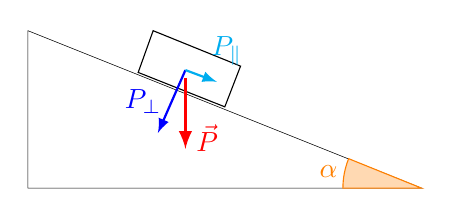
\begin{tikzpicture}
    \draw[very thin] (0,0) -- (5,0) -- (0,2) -- cycle; % Triangle
    \draw[thin] (1.59, 2) -- (1.4, 1.47)  -- (2.5,1.033) -- (2.7, 1.55)  -- cycle; % Block
    \draw[-latex, very thick, red] (2, 1.4) -- (2, 0.5) node[pos=0.5, below right]{$\vec{P}$}; % P
    \draw[-latex, thick, blue] (2, 1.5) -- (1.65, 0.7)
      node[pos=0.5, left]{$P_\perp$}; % P_perp
    \draw[-latex, thick, cyan] (2, 1.5) -- (2.4, 1.35)
      node[pos=0.5, above right]{$P_\Vert$}; % P_par
    \filldraw[orange, fill=orange!30] (5,0) -- (4,0)  arc(180:158:1) -- cycle;
    \draw[orange] (5,0) +(170:1.2) node{$\alpha$}; % Arc
  \end{tikzpicture}
\end{center}
\begin{equation*}
  \mathcolor{blue}{P_\perp} = \mathcolor{red}{P}\cos\mathcolor{orange}{\alpha}
\end{equation*}
\begin{equation*}
  \mathcolor{cyan}{P_\Vert} = m\cdot a_x = \mathcolor{red}{P}\sin\mathcolor{orange}{\alpha}
\end{equation*}
\begin{equation*}
  a_x = g\sin\mathcolor{orange}{\alpha}
\end{equation*}
\hyperref[tab:g]{$g$}: $9.81\,\text{m/s}^2$\\
$m$: massa del corpo\\
$a_x$: accelerazione sul piano inclinato\\
$\mathcolor{red}{\vec{P}}$: vettore della forza peso. Si noti che $\mathcolor{red}{P}$ è il suo 
modulo\\
$\mathcolor{orange}{\alpha}$: alzo del piano

\subsection{Funi e carrucole}
\begin{center}
  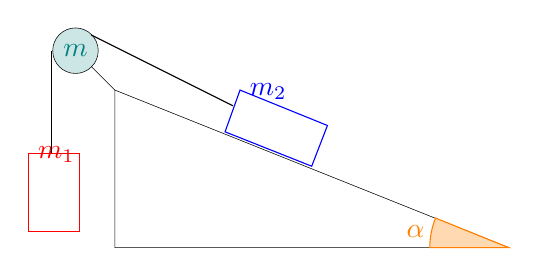
\begin{tikzpicture}
    \draw[very thin] (0,0) -- (5,0) -- (0,2) -- cycle; % Triangle
    \filldraw[orange, fill=orange!30] (5,0) -- (4,0)  arc(180:158:1) -- cycle;
    \draw[orange] (5,0) +(170:1.2) 
      node{$\alpha$}; % Arc
    \filldraw[fill=teal!20, very thin] (-0.5,2.5) circle (0.289) 
      node[teal]{$m$}; 
    \draw[very thin] (-0.3,2.3) -- (0,2); 
    \draw[red] (-1.1,1.2)--(-0.45,1.2)--(-0.45,0.2)--(-1.1,0.2)--cycle
      node[below=0.5,right]{$m_1$};
    \draw (-0.3,2.7)--(1.5,1.8);
    \draw (-0.8,1.2)--(-0.8,2.5);
    \draw[thin,blue] (1.59, 2) -- (1.4, 1.47)  -- (2.5,1.033) -- (2.7, 1.55) -- cycle 
      node[below=0.5,right]{$m_2$}; % Block
  \end{tikzpicture}
\end{center}
\begin{equation*}
  a = \frac{\mathcolor{red}{m_1}g - \mathcolor{blue}{m_2}g\sin\mathcolor{orange}{\alpha}}
  {\mathcolor{red}{m_1}+\mathcolor{blue}{m_2} + \frac{\mathcolor{teal}{m}}{2}}
\end{equation*}
Si noti che questa formula è particolare per questo caso. Si noti anche che 
$\dfrac{\mathcolor{teal}{m}}{2}$ è
da aggiungere solo se la massa della carrucola non è trascurabile.\\
Per una formula più generale si usi
\begin{equation*}
  a= \frac{\sum \vec{F}}{\sum m}
\end{equation*}
Per gli esercizi relativi a queste tre sottosezioni, si vada a pagina~\pageref{ex:dinamica:piano}.
\label{subsec:dinamica:piano}

\subsection{Forza centripeta e centrifuga}
Una corpo che si muove di moto circolare uniforme ha un accelerazione centripeta $a_c$, la forza 
centripeta perciò è:   
\begin{equation*}
  F_c =m\cdot a_c= m\cdot\frac{v^{2}}{r}
\end{equation*}
$v$: velocita del corpo\\
$r$: distanza tra il corpo e il centro della circonferenza
\begin{center}	
  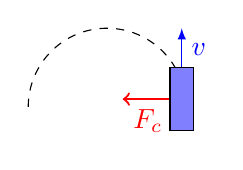
\begin{tikzpicture}
    \draw[black,dashed] (-1,-0.1) arc [start angle = 180, end angle = 0,
      x radius = 1, y radius = 1];
    \draw[<-,thick,red] (0.2,0) -- (1,0)
      node[pos=0.4, below]{$F_c$};
    \draw[-latex, blue] (0.95,0) -- (0.95, 0.9)
      node[pos=0.7, right]{$v$};
    \filldraw[fill=blue!50] (0.8,-0.4) rectangle (1.1,0.4);	
  \end{tikzpicture}
\end{center}
Una macchina dunque in curva non uscirà di strada se 
\begin{equation*}
  m\cdot\frac{v^{2}}{r} \leq \mu_s\cdot F_p
\end{equation*}
$\mu_s$: attrito statico\\
$F_p$: forza premente\\ [\baselineskip]

La "forza centrifuga" è invece solo una forza apparente che sembra esistere nel sistema di 
riferimento non inerziale del corpo in movimento che ha modulo opposto alla forza centripeta.\\
I sistemi possono essere essere analizzati come sistemi inerziali in cui 
\begin{equation*}
  \sum \text{Forze}=F_{\text{centripeta}}
\end{equation*}
o sistemi non-inerziali in cui 
\begin{equation*}
  \sum \text{Forze}=0
\end{equation*}
e in cui la $F_{\text{centrifuga}}$ è una delle forze.

\subsection{Momento}
Un corpo rigido è in equilibrio se $\sum M_o=0$.\\ Il momento($M_0$) è l'efficacia di una forza 
nel far ruotare un corpo intorno ad un punto ed è definito come   
\begin{equation*}
  M=Fd\cos (\alpha)
\end{equation*}
$F$: forza \\
$d$: distanza dal punto fulcro O \\ [\baselineskip]
Una forza è definita negativa se fa ruotare in senso orario il corpo, positiva se lo fa ruotare in
senso antiorario.\\
Prendiamo per esempio una leva
\begin{center}
  \begin{tikzpicture}[scale=2]
    \draw[black,thick](-1.5,-5)--(1.3,-5);
    \draw[red,->](-1.5,-5)--(-1.7,-4);
    \draw[red,dashed](-1.5,-5)--(-1.5,-4);
    \node[red] at (-1.56,-4.4) {$\alpha$};
    \draw[olive,->](1.3,-5)--(1,-4.1);
    \draw[olive,dashed](1.3,-5)--(1.3,-4.1);
    \node[olive] at (1.24,-4.57) {$\beta$};
    \draw [blue,->](-0.1,-5)--(-0.1,-5.5);
    \node [blue] at (0.1,-5.25){mg};
    \node at (-0.5,-5) {x};
    \node at (-0.5,-5.2) {O};
    \node at (-1.5,-5.1) {A};
    \node at (-0.1,-4.9) {M};
    \node at (1.3,-5.1) {C};
  \end{tikzpicture}
\end{center}
in cui per esserci equilibrio $\sum M_o=0$ dunque
\begin{equation*}
  -F_A AO\cos \alpha -mg MO+F_C CO\cos \beta=0
\end{equation*}
Va notato che spesso il peso della leva viene trascurato e la formula di conseguenza per 
l'equilibrio è
\begin{equation*}
  \vec{F_A} AO = \vec{F_C} CO
\end{equation*}
La risultante di due forze su un corpo ha intensità pari alla somma delle due forze  e il verso 
della forza con intensità maggiore  
\begin{center}
  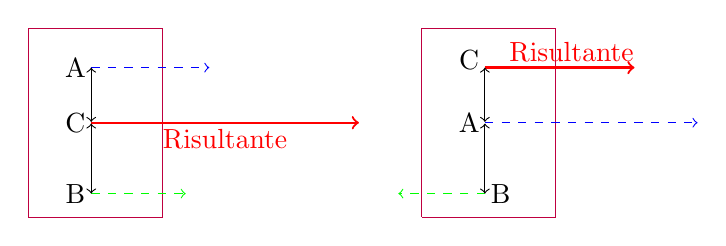
\begin{tikzpicture}
    \draw[purple] (0,0)--(0,2.4)--(1.7,2.4)--(1.7,0)--(0,0);
    \draw[blue,->,dashed] (.8,1.9)--(2.3,1.9);
    \draw[green,->,dashed] (.8,0.3)--(2,0.3);
    \draw[red,->,thick] (.8,1.2)--(4.2,1.2);
    \draw [<->] (.8,1.9)--(.8,1.21);
    \draw [<->] (.8,1.19)--(.8,0.3);
    \node at (.6,1.9) {A};
    \node at (.6,1.2) {C};
    \node at (.6,0.3) {B};
    \node at (2.5,1)[red] {Risultante};
    \draw[purple] (5,0)--(5,2.4)--(6.7,2.4)--(6.7,0)--(5,0);
    \draw[blue,->,dashed] (5.8,1.2)--(8.5,1.2);
    \draw[green,->,dashed] (5.8,0.3)--(4.7,0.3);
    \draw[red,->,thick] (5.8,1.9)--(7.7,1.9);
    \draw [<->] (5.8,1.9)--(5.8,1.21);
    \draw [<->] (5.8,1.19)--(5.8,0.3);
    \node at (5.6,2) {C};
    \node at (5.6,1.2) {A};
    \node at (6,0.3) {B};
    \node at (6.9,2.1)[red] {Risultante};  
  \end{tikzpicture}
\end{center}
e si dimostra che 
\begin{equation*}
  AC:CB=F_B:F_A
\end{equation*}


\subsection{Lavoro, Energia e Potenza}\label{subsec:dinamica:potenziale}
Il \emph{lavoro} è una grandezza scalare ed il prodotto della forza applicata sul corpo e lo 
spostamento del corpo.\\L'unita di misura del \emph {lavoro} è il Joule(J).
\begin{equation*}
  \vec{L} = \vec{F} \cdot \mathcolor{blue}{\vec{x}}
  = F\cdot \textcolor{blue}{x} \cdot \cos\mathcolor{red}{\alpha}
\end{equation*}
\begin{center}
  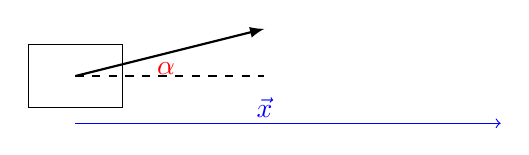
\begin{tikzpicture}
    \draw  (0,0) rectangle (1.2,0.8);
    \draw [-latex,thick] (0.6,0.4)--(3,1);
    \draw [dashed](0.6,0.4)--(3,0.4);
    \node [red] at (1.75,0.5) {$\alpha$};
    \draw [->,blue](0.6,-0.2)--(6,-0.2);
    \node[blue] at (3,0){$\vec {x}$};
  \end{tikzpicture}
\end{center}
La \emph {potenza} invece misura quanto rapidamente viene compiuto lavoro, ha come unita di misura 
il Watt(W).
\begin{equation*}
  P = \frac{L}{t}
\end{equation*}
$t$: tempo \\ [\baselineskip]
La potenza di una forza $F$ che agisce su un corpo che si muove di moto rettilineo uniforme è
\begin{equation*}
  P=F\cdot v
\end{equation*}
$v$: velocità del corpo\\ [\baselineskip]
L'\emph{enegia cinetica} è l'energia di un corpo in movimento.\\
\begin{equation*}
  E_c = \frac{1}{2}mv^2
\end{equation*}
$m$: massa del corpo\\
$v$: velocità del corpo\\ [\baselineskip]
Inoltre la differenza di Energia cinetica è :
\begin{equation*}
  \Delta E_{cinetica}=Lavoro
\end{equation*}
L'\emph{Energia potenziale} è l'energia che un corpo (sulla terra) acquisisce allontanandosi dalla
superficie. L'energia potenziale indica quanta energia un corpo (se fermo) al massimo può generare.
\begin{equation*}
  U = mgh
\end{equation*}
$m$: massa del corpo\\
$h$: distanza dalla superficie terrestre\\ [\baselineskip]
Si può dimostrare che
\begin{equation*}
  -\Delta U = L
\end{equation*}
è dunque l'unita di misura dell'energia è il Joule.\\ [\baselineskip]
L'energia meccanica $E$ è definita come
\begin{equation*}
  E=E_{cinetica}+E_{potenziale}
\end{equation*}
è stato dimostrato sperimentalmente che l'energia meccanica si conserva (quando è assente 
l'attrito)
\begin{equation*}
  U_1 + E_{cinetica1} = U_2 + E_{cinetica2}
\end{equation*}
Negli esercizi sarà particolarmente utile in quanto permette di trovare la velocità o l'altezza di
un corpo con calcoli semplici.\\ [\baselineskip]

\subsubsection{Legge di Hooke e energia elastica}
Una molla compressa o allungata esercita una forza elastica e possiede energia potenziale. È da 
notare che i due estremi di una molla esercitano forze uguali ma contrarie.
\begin{equation*}
  \vec{F} = -k\vec{x}
\end{equation*}
\begin{equation*}
  U_e = \frac{1}{2}k\Delta x^2
\end{equation*}
$k$: costante elastica della molla\\
$\vec{x}$: spostamento dalla direzione di riposo\\[\baselineskip]

\subsection{Oscillatore armonico}
\begin{center}
  \begin{tikzpicture}
    \draw (0,0) -- (5,0);
    \draw[pattern=north east lines] (0,0) -- (1,0) -- (1,1) -- (0,1);
    \draw[decoration={coil},decorate] (1,0.5) -- (3,0.5);
    \draw (3.5,0.5) circle (0.5);
  \end{tikzpicture}
\end{center}
Quando questa massa si muove di una distanza $x_0$ e poi viene rilasciata, tenderà a tornare alla
posizione originale. Posto $\omega=\sqrt{\frac{k}{m}}$ si avrà che
\begin{equation*}
  x=x_0\cos\omega t
\end{equation*}
dove $k$ è la costante della molla.

\subsection{Quantità di moto e teorema dell'impulso}\label{subsec:dinamica:impulso}
\label{subsec:qtaMoto}
\begin{equation*}
  \vec{q} = m\vec{v}
\end{equation*}
\begin{equation*}
  \vec{I} = \Delta \vec{q} = \vec{F}\Delta t
\end{equation*}
$m$: massa del corpo\\
$\vec{v}$: velocità del corpo\\
$\vec{F}$: forza applicata sul corpo\\
$t$: tempo\\[\baselineskip]
La quantità di moto si conserva sempre nel tempo.Quando ad esempio un vaso cade e si rompe, la 
somma delle quantità di moto di tutti i frammenti deve essere pari a quella del vaso all'impatto; 
questo spiega perchè i frammenti più leggeri sono quelli che si allontanano di più.\\
La quantità di moto indica la forza necessaria a fermare un oggetto in movimento in un secondo.\\
[\baselineskip]
Si ricordi che
\begin{equation*}
  \sum \vec{q} = \text{ costante nel tempo}
\end{equation*}
\begin{center}
  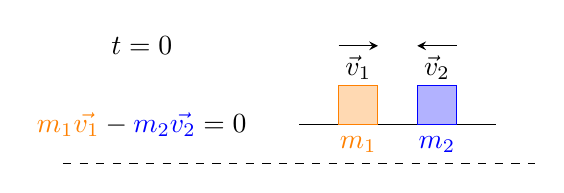
\begin{tikzpicture}
    \draw (0,0) -- (2.5,0);
    \filldraw[orange, fill opacity = 0.3] (0.5,0) -- ++(0.5,0) -- ++(0,0.5) -- ++(-0.5,0) -- cycle;
    \filldraw[blue, fill opacity = 0.3] (1.5,0) -- ++(0.5,0) -- ++(0,0.5) -- ++(-0.5,0) -- cycle;

    \draw[-stealth] (0.5,1) -- ++(0.5,0)
      node[pos=0.5, below]{$\vec{v}_1$};
    \draw[stealth-] (1.5,1) -- ++(0.5,0)
      node[pos=0.5, below]{$\vec{v}_2$};
    \node[orange] at (0.75,-0.25){$m_1$};
    \node[blue] at (1.75,-0.25){$m_2$};
    \node at (-2,0){$\mathcolor{orange}{m_1\vec{v_1}}-\mathcolor{blue}{m_2\vec{v_2}} = 0$};
    \node at (-2,1){$t=0$};
    \draw[dashed] (-3,-0.5) -- (3,-0.5);
  \end{tikzpicture}
\end{center}
\begin{center}
  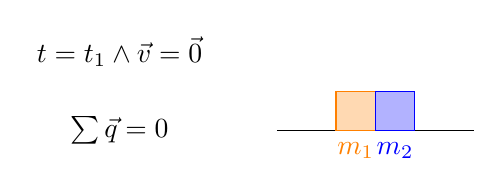
\begin{tikzpicture}
    \draw (0,0) -- (2.5,0);
    \filldraw[orange, fill opacity=0.3] (0.75,0) -- ++(0.5,0) -- ++(0,0.5) -- ++(-0.5,0) -- cycle;
    \filldraw[blue, fill opacity = 0.3] (1.25,0) -- ++(0.5,0) -- ++(0,0.5) -- ++(-0.5,0) -- cycle;

    \node[orange] at (1,-0.25){$m_1$};
    \node[blue] at (1.5,-0.25){$m_2$};

    \node at (-2,0){$\sum\vec{q}=0$};
    \node at (-2,1){$t=t_1\land\vec{v}=\vec{0}$};
  \end{tikzpicture}
\end{center}
Per gli esercizi si vada a pagina~\pageref{ex:impulso}.

\subsection{Urti}\label{subsec:dinamica:urti}
Si distinguono 2 tipi di urti: \emph{elastici} e \emph{anaelastici}.\\[\baselineskip]
Negli urti \emph{elastici} i due corpi collidono ma rimangono separati. Ad esempio due palle
da biliardo.\\
Negli urti \emph{anaelastici} i due corpi che collidono rimangono attaccati l'uno all'altro,
come nel caso di un pesce che ne mangia un altro o di un proiettile che colpisce un sacco.\\

Per gli esercizi si vada a pagina~\pageref{ex:urti}.

\subsubsection{Elastico}
\begin{equation*}
  v_{1_f} = \frac{v_{1_i}\left(m_1-m_2\right) + 2m_2v_{2_i}}{m_1+m_2}
\end{equation*}
\begin{equation*}
  v_{2_f} = \frac{2m_1v_{1_i} + v_{2_i}\left(m_2-m_1\right)}{m_1+m_2}
\end{equation*}
$_1$: relativo al primo corpo\\
$_2$: relativo al secondo corpo

\subsubsection{Anaelastico}
\begin{equation*}
  m_1v_1 + m_2v_2 = v(m_1+m_2)
\end{equation*}
$_1$: relativo al primo corpo\\
$_2$: relativo al secondo corpo\\
$v$: velocità finale

\subsubsection{Proiettile contro un corpo}
Se un proiettile colpisce un sacco e rimane bloccato, il baricentro del sacco si alzerà di 
un'altezza $h$.
\begin{center}
  \begin{tikzpicture}
    \coordinate (ROT) at (1, 2);
    \coordinate (CenterB1) at ($(ROT) + (0, -1.5)$);
    \coordinate (CenterB2) at ($(ROT) + (2, -1.3)$);
    \coordinate (CenterP) at (0,0.5);

    \draw (ROT) -- ($(CenterB1) + (0, 0.5)$);
    \draw (ROT) -- ($(CenterB2) + (-0.5, 0.5)$);

    \draw[very thin] ($(CenterB1) + (-0.5, -0.5)$) -- ($(CenterB1) + (-0.5, +0.5)$) --
      ($(CenterB1) + (0.5, 0.5)$) -- ($(CenterB1) + (0.5, -0.5)$) -- cycle % Box1
      node[pos=0.5, above, red]{$M$};
    \draw[very thin,
      densely dashed] ($(CenterB2) + (-0.5, -0.5)$) -- ($(CenterB2) + (-0.5, +0.5)$) --
      ($(CenterB2) + (0.5, 0.5)$) -- ($(CenterB2) + (0.5, -0.5)$) -- cycle;
    \draw[densely dotted] (CenterB1) -- ($(CenterB1) + (2.5, 0)$);
    \draw[blue, thick] ($(CenterB1) + (2, 0)$) -- (CenterB2)
      node[pos=0.5, right]{$h$};
    \draw ($(CenterP) + (-0.2, -0.1)$) -- ($(CenterP) + (0.2, -0.1)$) --
      ($(CenterP) + (0.2, 0.1)$) -- ($(CenterP) + (-0.2, 0.1)$) -- cycle
      node[teal, below]{$\vec{v_p}$}
      node[teal, above left]{$m$};
  \end{tikzpicture}
\end{center}
\begin{equation*}
  \mathcolor{blue}{h} = 
  \frac{\mathcolor{teal}{v_p}^2\mathcolor{teal}{m}^2}{2g\left(\mathcolor{red}{M} +
  \mathcolor{teal}{m}\right)^2}
\end{equation*}
$v_p$: velocità del proiettile\\
$h$: altezza finale del sacco

\subsubsection{Urti obliqui}
Vi è un urto obliquo quando due corpi collidono e si muovono in direzioni diverse.
\begin{center}
  \begin{tikzpicture}
    \coordinate (C1) at (-1,0);
    \coordinate (C2) at (1,0);
    \coordinate (D) at (1.3,0);
    \coordinate (E1) at (2.5, 0.5);
    \coordinate (E2) at (2.5, -0.7);

    \draw[orange] (C1) circle (0.25)
      node[]{A};
    \draw[teal] (C2) circle (0.25)
      node[]{B};
    \draw[-latex] ($(C1) + (0.35,0)$) -- ($(C2) + (-0.35,0)$);
    \draw[-latex, dashed] (D) -- ($(D) + (1.5, 0)$);
    \draw[-latex] (D) -- (E1);
    \draw[-latex] (D) -- (E2);
    \filldraw[red, fill=red!30] (D) -- ($(D) + (0.4,0)$) arc(0:9:1) -- cycle;
    \draw[red] (D) +(10:0.5) node{$\alpha$};
    \filldraw[blue, fill=blue!30] (D) -- ($(D) + (0.4,0)$) arc(0:-13:1) -- cycle;
    \draw[blue] (D) +(-13:0.7) node{$\beta$};
  \end{tikzpicture}
\end{center}
\begin{equation*}
  \vec{q}
  \begin{cases*}
    \mathcolor{orange}{m_A}\mathcolor{orange}{v_a}\sin\mathcolor{red}{\alpha}-
    \mathcolor{teal}{m_B}\mathcolor{teal}{v_b}\sin\mathcolor{blue}{\beta} = v_0m\\
    \mathcolor{orange}{m_A}\mathcolor{orange}{v_a}\cos-\mathcolor{red}{\alpha}-
    \mathcolor{teal}{m_B}\mathcolor{teal}{v_b}\cos-\mathcolor{blue}{\beta} = 0
  \end{cases*}
\end{equation*}
$v_0$: velocità iniziale del corpo $A$\\
$v_A$: velocità finale del corpo $A$\\
$v_B$: velocità finale del corpo $B$

\subsection{Centro di Massa}\label{subsec:dinamica:cm}
Il centro di massa è un punto in un corpo. In quel punto si potrebbe concentrare tutta la massa del
corpo per renderlo puntiforme.\\
Le formule riportate possono valere per tutte le dimensioni, qui però
verrà presa in considerazione solo una per semplicità.

\begin{alignat*}{3}
  x &= \frac{\sum\limits_{i=0}^{n} m_ix_i}{\sum\limits_{i=0}^{n} m_i} &\quad
  \vec{v}_{CM} &= \frac{\sum\limits_{i=0}^{n} m_i\vec{v_i}}{\sum\limits_{i=0}^{n} m_i} &\quad
  \vec{a}_{CM} &= \frac{\sum\limits_{i=0}^{n} m_i\vec{a_i}}{\sum\limits_{i=0}^{n} m_i}
\end{alignat*}
Per gli esercizi si vada a pagina~\pageref{ex:cm}.

\subsection{Momento Angolare e Momento d'Inerzia}\label{subsec:dinamica:inerzia}
Il momento angolare ($\vec{L}$) è la quantità di moto per le rotazioni.\\
Al concetto di \emph{momento angolare} si accompagna anche quello di \textbf{momento di inerzia}. 
L'inerzia ($I$) indica quanto un corpo si oppone alla rotazione.\\
\begin{equation*}
  \vec{L} = \vec{r} \times \vec{q}
\end{equation*}
Da qui si nota la relazione stretta con la \hyperref[subsec:qtaMoto]{Quantità di moto}.
\begin{equation*}
  L = mr^2\omega = I\omega
\end{equation*}
\begin{equation*}
  I = mr^2 = \sum\limits_{i=0}^{n}m_ir_i^2
\end{equation*}
$m$: massa del corpo\\
$\omega$: velocità angolare\\
$q$: quantità di moto\\[\baselineskip]
Se un corpo ruota rispetto ad un asse parallelo a quello passante per il centro di massa e la distanza
tra i due assi è $d$ e la massa totale $m$, è
\begin{equation*}
  I = I_{CM}+md^2
\end{equation*}
\begin{center}
  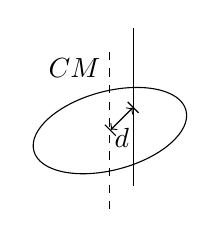
\begin{tikzpicture}
    \draw[dashed] (0,1) -- (0,-1)
      node[pos=0.1, left]{$CM$};
    \draw (0.3,1.3) -- (0.3,-0.7);
    \draw[|<->|] (0,0) -- (0.3,0.3)
      node[pos=0.5,below]{$d$};
    \draw[rotate around={15:(0,0)}] ellipse(1 and 0.5);
  \end{tikzpicture}
\end{center}
In aggiunta al momento angolare e al momento di inerzia, c'è la \textbf{forza angolare} ($\vec{M}$).
Molto semplicemente è definita
\begin{equation*}
  \vec{M} = \vec{r}\times\vec{F}
\end{equation*}
\begin{equation*}
  \vec{M} = I\vec{\alpha}
\end{equation*}
\begin{equation*}
  \Delta L = M\Delta t
\end{equation*}
$\alpha$ identifica \hyperref[subsec:mrua]{l'accelerazione angolare}.\\

\subsubsection{Teorema di König}
Il teorema di König descrive l'energia cinetica in un moto roto-traslato. Ad esempio una ruota che 
si muove sull'asfalto (ruota sul suo asse e trasla sull'asfalto).
\begin{equation*}
  E_c = \frac{1}{2} I\omega^2 + \frac{1}{2}mv_{CM}^2
\end{equation*}
$I$: inerzia\\
$\omega$: velocità angolare\\
$v_{CM}$: velocità del centro di massa\\[\baselineskip]
Per gli esercizi si vada a pagina~\pageref{ex:inerzia}.

\subsubsection{Tabella riassuntiva e di confronto}
\begin{center}
  \begin{tabular}{M{3cm} M{3cm}}
    \textbf{Traslatorio} & \textbf{Rotatorio}\\\hline
    $x=v_0t+\frac{1}{2}at^2$ & $\theta=\omega t+\frac{1}{2}\alpha t^2$\\\hline
    $a=\frac{\Delta v}{\Delta t}$ & $\alpha=\frac{\Delta\omega}{\Delta t}$\\\hline
    $F=ma$ & $M=I\alpha$\\\hline
    $q=mv$ & $L=I\omega$\\\hline
    $\Delta q=F\Delta t$ & $\Delta L = M\Delta t$\\\hline
    $E_c=\frac{1}{2}mv^2$ & $E_c=\frac{1}{2}I\omega^2$
  \end{tabular} 
\end{center}
